\mode*

\section{Introduction}%
\label{Introduction}

Alice is an activist who organizes a protest for some cause.
Eve is an autocrat who opposes Alice's cause.
Bob, Carol and many others participate in the protest against Eve.
One problem that has not yet been entirely solved is the crowd-counting 
problem, i.e.\ to verify how many participated in Alice's protest.
Our main goal is to provide a tool which prevents both Alice and Eve from 
cheating.

\mode<presentation>{%
\subsection{What's the problem?}
}

\begin{frame}<presentation>
  \begin{block}{The crowd-counting problem}
    \begin{itemize}
      \item Alice organizes a protest against Eve's regime.
      \item Bob, Carol and others show up.
      \item We want to know how many showed up to support Alice.
    \end{itemize}
  \end{block}
\end{frame}

\mode<presentation>{%
\subsection{Why is it a problem?}
}

\mode<presentation>{%
\begin{frame}
  \begin{figure}
    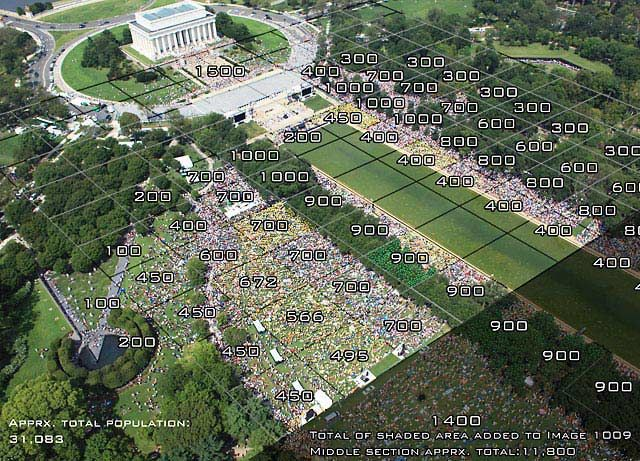
\includegraphics[height=0.9\textheight]{Jacobs-method.jpg}
  \end{figure}
\end{frame}

\begin{frame}
  \begin{example}
    \begin{itemize}
      \item Computer vision does object recognition.
      \item Requires photos/video that cover the entire location, all the time.
      \item This will count people twice.
    \end{itemize}
  \end{example}

  \pause{}

  \begin{example}
    \begin{itemize}
      \item Scan active mobile phones in the area.
      \item This requires some extra equipment.
      \item This catches bystanders who are not protesting.
    \end{itemize}
  \end{example}
\end{frame}
}

\mode<none>{%
\begin{frame}
  \begin{example}
    \begin{itemize}
      \item South Korea 2016~\cite{2016DemonstrationsInSeoul}:
        approximate count by imagery.
        \begin{description}
          \item[Organizers] 1\,000\,000
          \item[Police] 260\,000
        \end{description}

        \pause{}

      \item US 2017~\cite{2017WomensMarchesInUS}:
        sum up people's approximations.
      \item This makes it even difficult to estimate the error.
    \end{itemize}
  \end{example}
\end{frame}
}

After many demonstrations the count by police and that by the organizers 
differ\footnote{%
  This is actually quite natural, they have different goals.
  The organizers want to count everyone who ever participated.
  Police want to estimate the count at the peak of participation, due to crowd 
  control~\cite{2016DemonstrationsInSeoul}.
}, in some instances the difference can be hundreds of thousands.
There are numerous examples, e.g.\ the demonstrations in South 
Korea~\cite{2016DemonstrationsInSeoul}, Trump's 
inauguration~\cite{HowWillWeKnowTrumpInauguralCrowdSize} or the Women's Marches 
in the US~\cite{2017WomensMarchesInUS}, where there is difficulty in 
establishing the actual number of participants.
The methods for counting the crowds vary.
Most of the available methods lack precision, i.e.\ they have large error 
margins.
They can only give an estimate for a particular snapshot in time, e.g.\ at the 
peak of the event, not the cumulative participation count --- at least not 
without counting some people multiple times, which in turn increases the error 
of the estimation.
Finally, they also lack verifiability, i.e.\ everyone must trust the entity who
does the counting.
(We will discuss them in more detail in \cref{RelatedWork}.)

\begin{frame}<presentation>
  \begin{block}{Verifying protest participation}
    \begin{itemize}
      \item Alice organizes a protest against Eve's regime.
      \item Bob, Carol and others show up.

        \pause{}

      \item {\color{green} Alice wants to show that many support her cause.}

        \pause{}

      \item {\color{red} Eve wants to show that few support Alice's cause.}
      \item It's an adversarial setting!
      \item We need verifiable results.
    \end{itemize}
  \end{block}
\end{frame}

We can make one important observation about this problem that has seemingly 
been ignored in the past: it is an adversarial setting.
Alice the activist has an incentive to increase the tallied number of 
participants, whereas Eve (and possibly other interests) have an incentive to 
decrease the tallied number of participants.
In this case we have two options:
either we trust Alice or Eve, or we must verify their claims.
We aim for verifiable claims.
To solve this problem, we need a verifiable participation count which is 
protected from Sybil attacks.

\subsection{Combining electronic voting and location proofs}

In general, protesting is very similar to voting: both are many individuals 
expressing their opinion.
These opinions can be sensitive, hence we desire to have similar properties of 
verification and privacy for participation in a protest as there is for voting.

Voting has three requirements for 
verifiability~\cite{VerifyingPrivacyPropertiesOfVotingProtocols}.
\begin{itemize}
  \item Eligibility: anyone can verify that each vote cast is legitimate.
  \item Universal verifiability: anyone can verify that the result is according 
    to the cast votes.
  \item Individual verifiability: every voter can verify that their vote is 
    included in the result.
\end{itemize}
We translate the votes into \emph{proofs of participation}.
Universal and individual verifiability remain the same: anyone can verify the 
participation count by counting the proofs.
The eligibility requirement is slightly different:
for protests the eligibility requirement must include temporal and spatial 
eligibility, i.e.\ that each proof of participation satisfies some temporal and 
spatial relation to the protest.
In essence, the proof must bind the person to the time and location of the 
protest.
We will define these more formally in \cref{Verifiability}.

There are also three levels of 
privacy~\cite{VerifyingPrivacyPropertiesOfVotingProtocols}:
\begin{itemize}
  \item\label{VotePrivacy} Vote privacy: the voting does not reveal any 
    individual vote.
  \item\label{ReceiptFreeness} Receipt freeness: the voting system does not 
    provide any data that can be used as a proof of how the voter voted.
  \item\label{CoercionResistance} Coercion resistance: a voter cannot cooperate 
    with a coercer to prove the vote was cast in any particular way.
\end{itemize}
We note that we cannot improve the privacy of participating protesters, if they 
are caught during a protest there is nothing we can do.
But if they are not caught in the act, then using our proposed tool should not 
incur any additional risk.
Thus we will adapt the idea of receipt freeness (see \cref{Privacy} for a 
detailed definition) to the protest context.
In essence, upon completing the protocol, Eve cannot link Alice to Alice's 
participation proof --- even with Alice's cooperation.

\subsection{Contributions}

We propose a protocol which provides a way for protests to be securely verified.
Additionally, this verification system does not incur any additional risk to 
protesters' privacy than participating in the physical protest itself.

\dots

Sometimes Eve's authoritarian regime wants to organize a pro-regime protest to 
demonstrate its \enquote{wide 
  support}~\cite[e.g.][]{AlJazeeraOnVenezuela2017,VenezuelanStateWorkersCalledToParticipate}.
If we rely on government-issued credentials, we cannot prevent the government 
from performing Sybil attacks --- since it can issue arbitrarily many 
\enquote{valid} credentials.
This means that we cannot verify any pro-government protests.

